\subsubsection{Shock pool}
\label{sec.tests.shockpool}

The next problem is similar to the last one but instead examines how a shock with a Mach number of 2 passes in and out of a static refined region (again defined from $z=0.25$ to 0.75).  The density and pressure in the domain is initially set equal to 1.0 with zero velocity.  At $t=0$ the left boundary is set with the density, pressure and velocity appropriate for a $\mathcal{M}=2$ shock wave.

In Figure~\ref{fig.shockpool}, we show the evolution of the shock wave at three times, again corresponding to just before entering the refine region (left column), after entering the refined region (center), and after exiting the refined region (right).  We examine the same set of three solvers as in the previous test problem.

Beginning with PPM (top row of Figure \ref{fig.shockpool}), we see that this method captures the shock in a small number of zones with only a small amount of oscillation.  Upon entering the refined region, the shock finds itself broader than the natural width of the scheme (since the cell spacing is decreased by a factor of 2), and so the shock front contracts, causing a slight entropy perturbation in the post-shock gas. 

For Zeus (middle row of Figure~\ref{fig.shockpool}), the shock is broadened because of artificial viscosity and there are slightly more post-shock oscillations, although again quite mild.  The impact of entering and exiting the refined region is somewhat larger than in PPM; however, the most noticeable difference is the incorrect position of the shock front. This is due to the fact that the scheme is not energy-conserving (see also the Sedov problem, below), and has very little to do with the passage through the refined region.

Finally, the MUSCL scheme produces a shock which is intermediate in width between the two previous cases.  This method is energy conserving and so correctly reproduces the shock speed.  The oscillations are mild except for the cell immediately outside of the refined region upon exiting.

\begin{figure}
\begin{center}
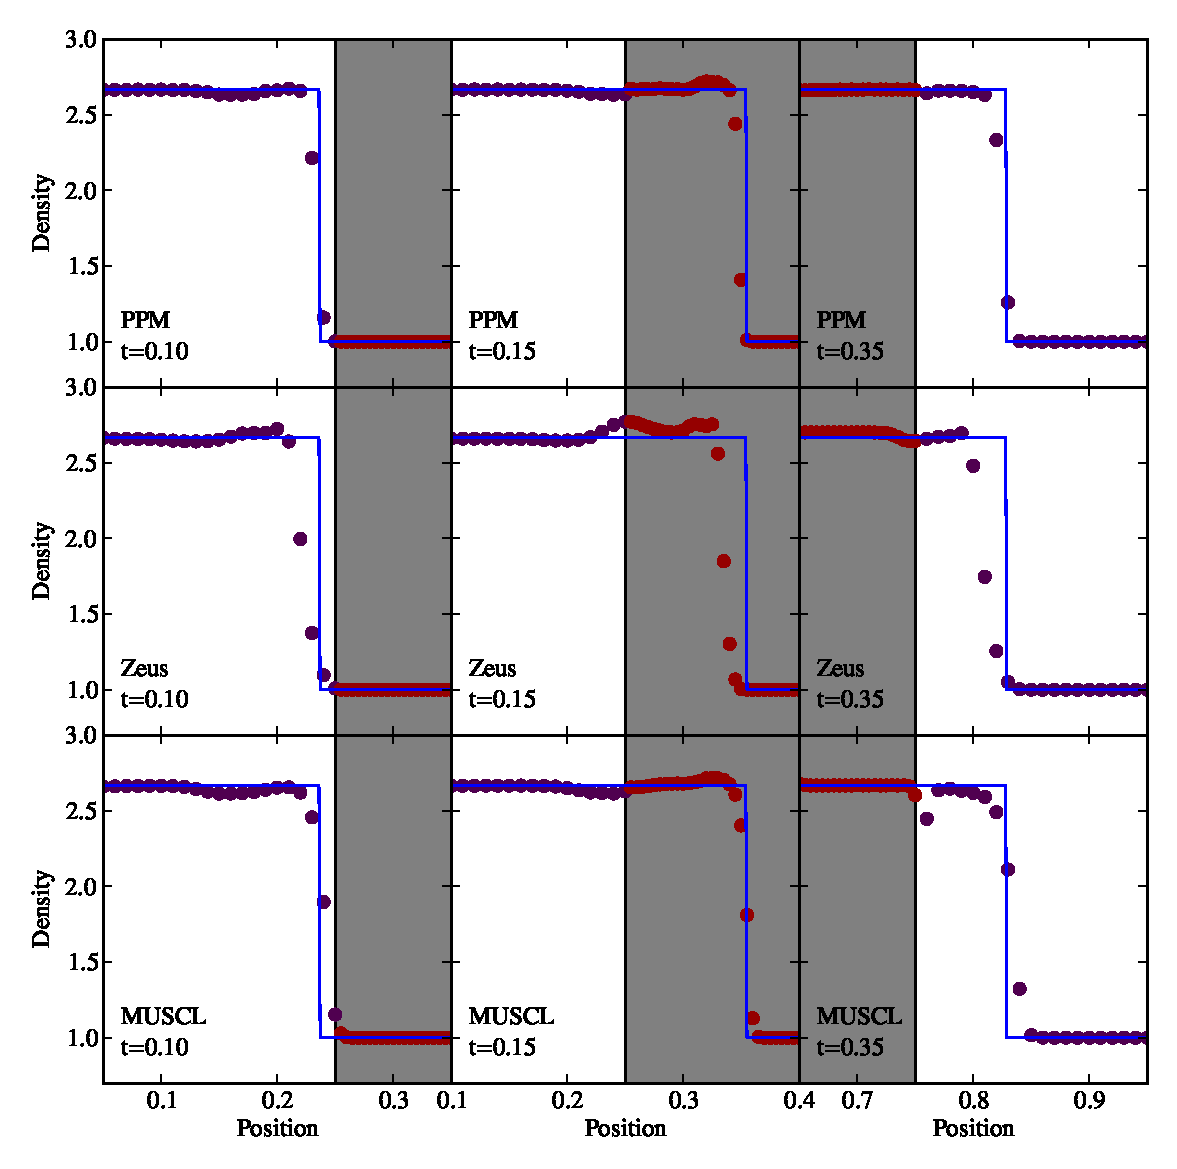
\includegraphics[width=0.8\textwidth]{figures/ShockPool}
\caption{This plot shows, for each column, three snapshots at $t=0.1, 0.15$ and 0.35 of a $\mathcal{M}=2$ shock as it propagates through the grid with a static refined region extends from $x = 0.25$ to 0.75 (shown in grey in each panel).   Each row shows the result for a different solver (PPM/Zeus/MUSCL from top to bottom).  The solid line shows the analytic solution.  Note that we focus each panel on a small region of the entire domain to better show the shock front.}
\label{fig.shockpool}
\end{center}
\end{figure}
